\begin{figure*}[t!]
    \begin{minipage}[t]{.33\textwidth}
    %   \centering
      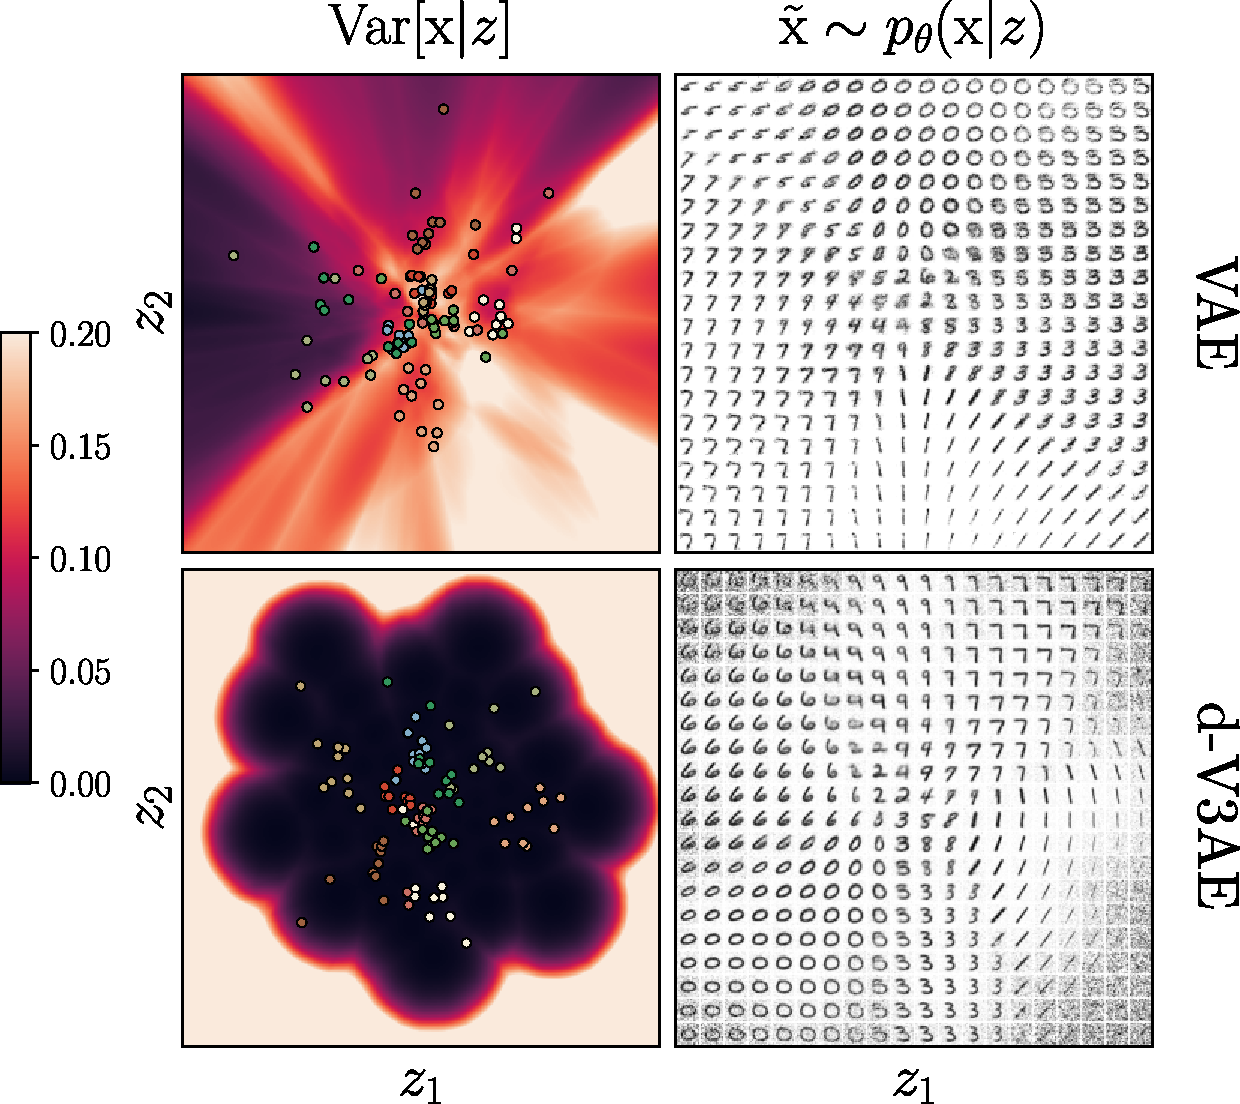
\includegraphics[width=\textwidth]{assets/vae_variance_plots.pdf} % 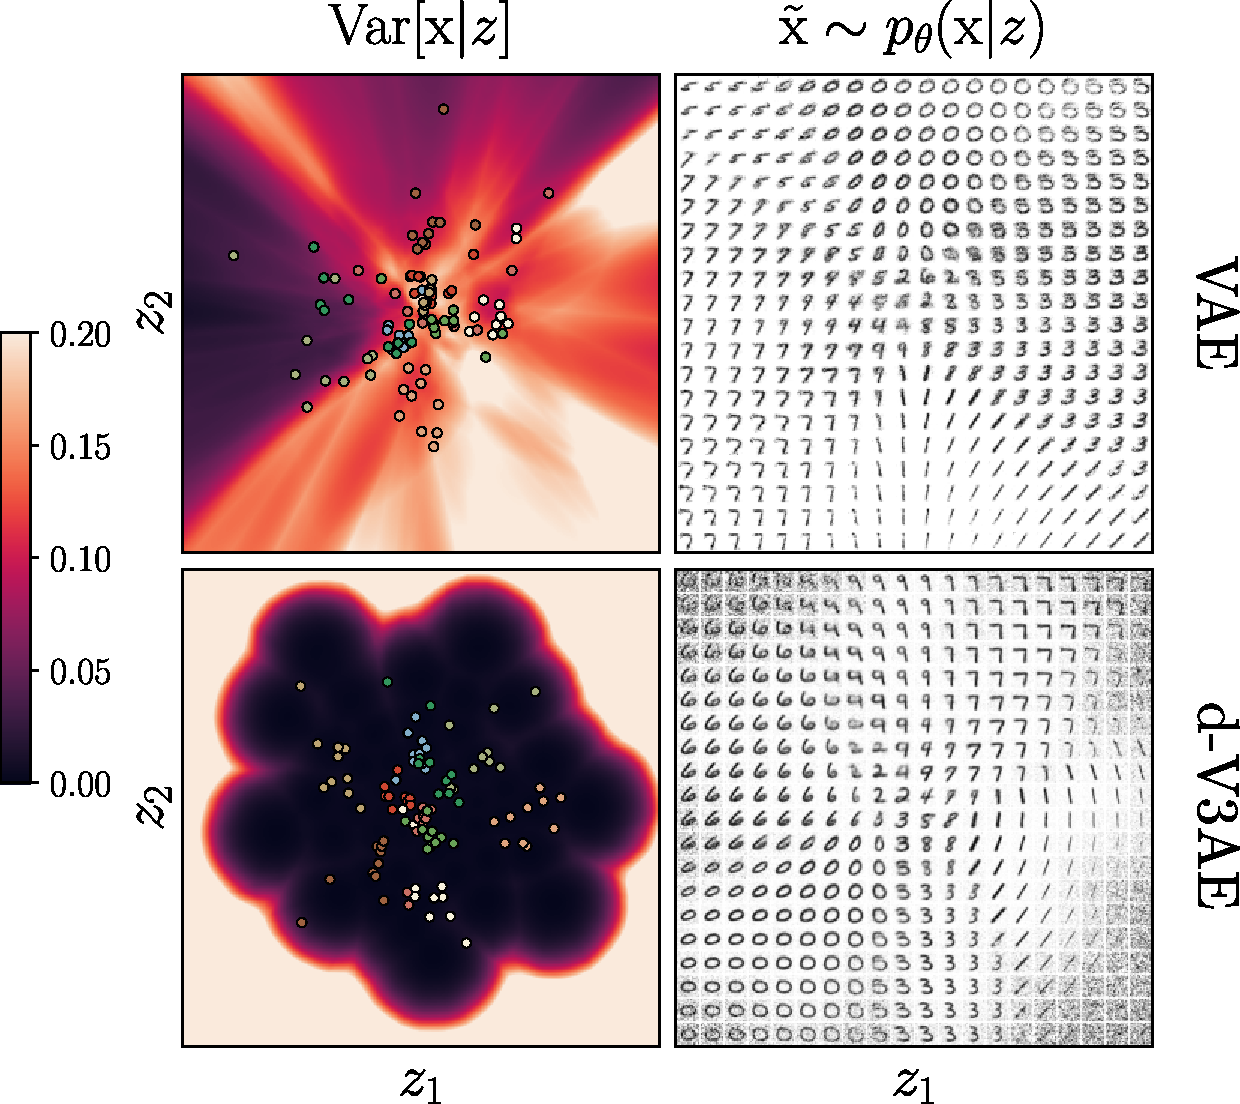
\includegraphics[height=5cm]{assets/vae_variance_plots.pdf}
      \vspace{-2.5mm}
      \captionof{figure}{Decoder's aggregated variance (left) and generated samples (right) from the latent space. Coloured points correspond to latent representations of test data, with per-class colours.}
      \label{fig:vae_variance_plots}
    \end{minipage}%
    \hspace{.02\textwidth}
    \begin{minipage}[t]{.39\textwidth}
        \vspace{-5cm}
    %   \centering
      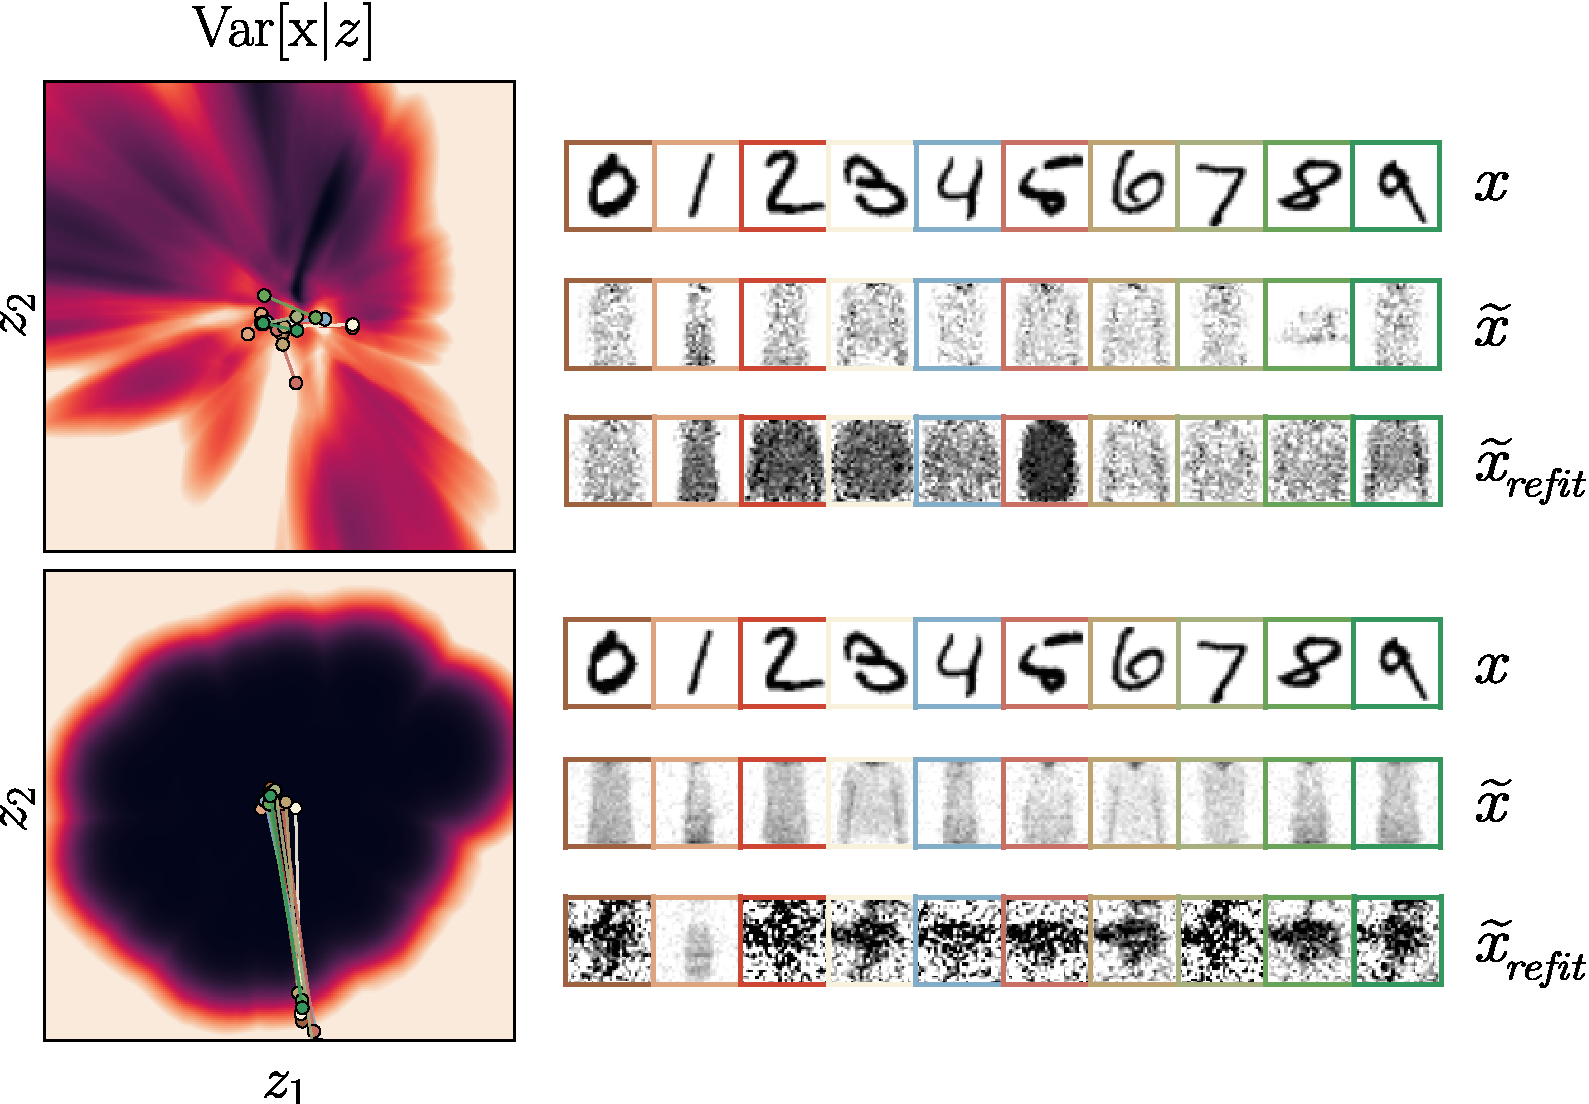
\includegraphics[width=\textwidth]{assets/re_encoding_plot.pdf} %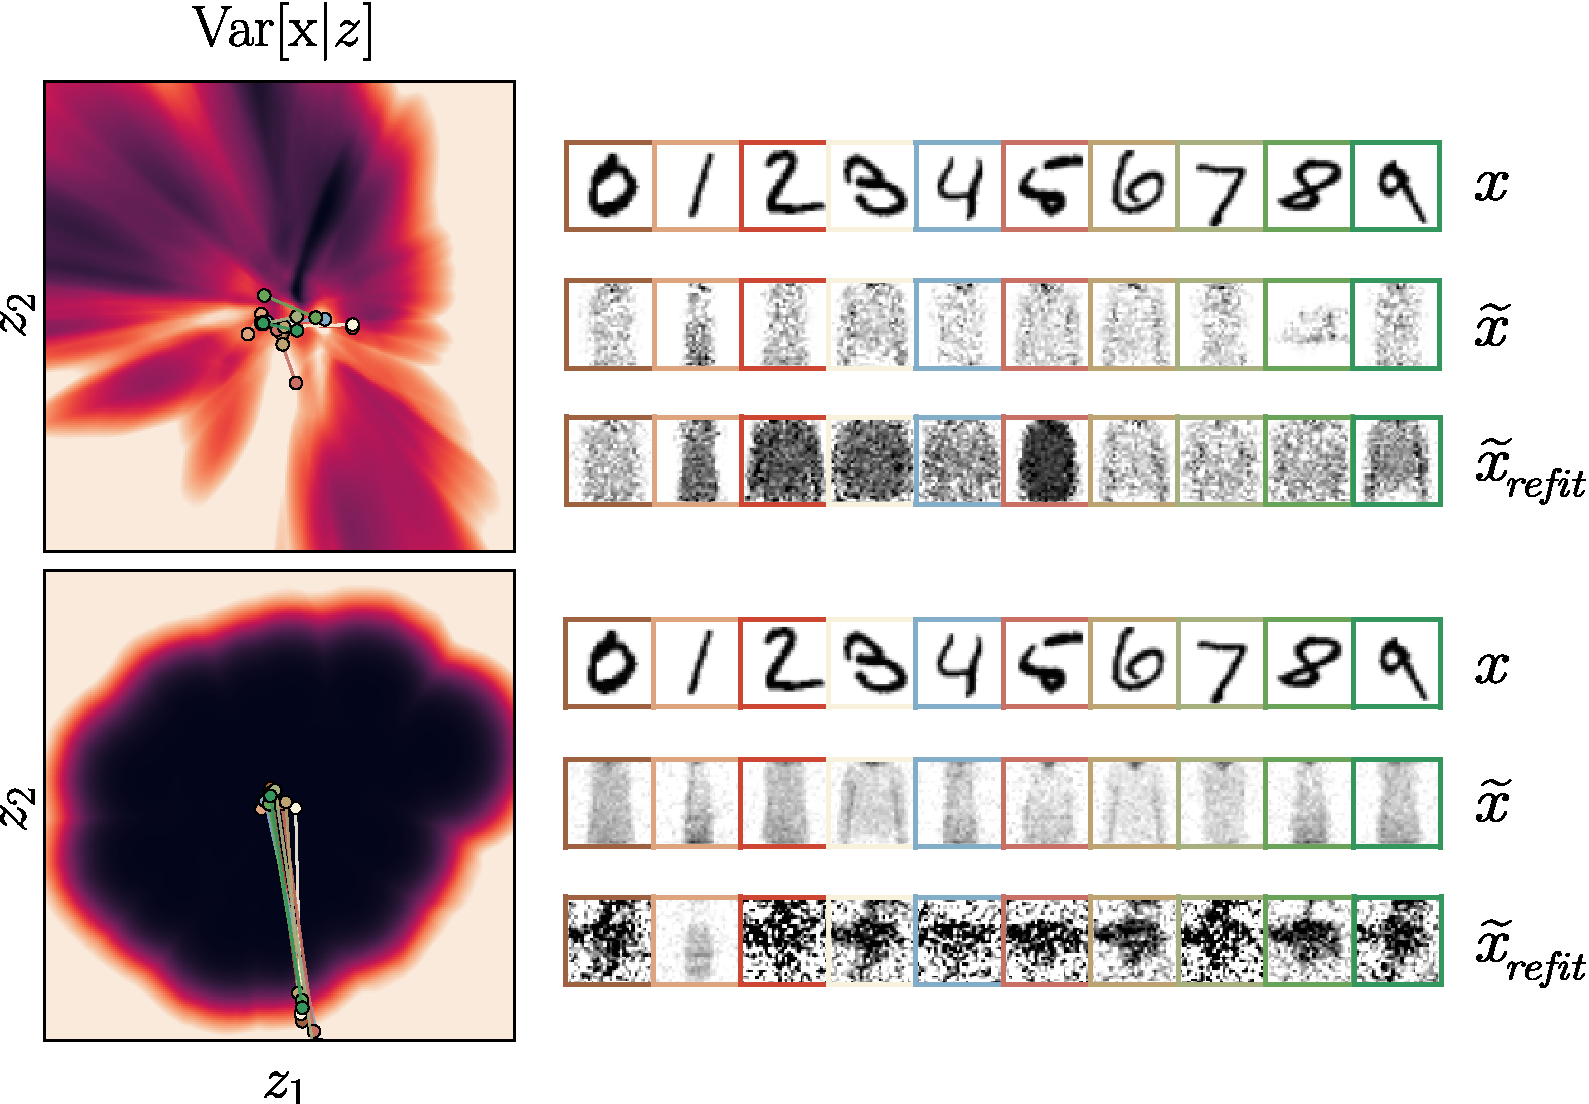
\includegraphics[height=5.05cm]{assets/re_encoding_plot.pdf}
      \vspace{-5.5mm}
      \captionof{figure}{Effect of encoder refitting on the latent representations (left) and corresponding samples (right). OOD inputs (first rows, $x$) initially result in in-distribution samples (second rows, $\tilde{x}$). The refitted encoder displaces the encodings (coloured trajectories), modifying the generated samples (third rows, $\tilde{x}_{\text{refit}}$).}
      \label{fig:re-encoding}
    \end{minipage}
    \hspace{.02\textwidth}
    \begin{minipage}[l]{.2\textwidth}
        \centering
        \vspace{-1.8cm}
        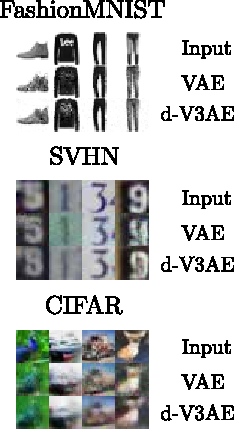
\includegraphics[width=4cm]{assets/show_vae_samples.pdf} % 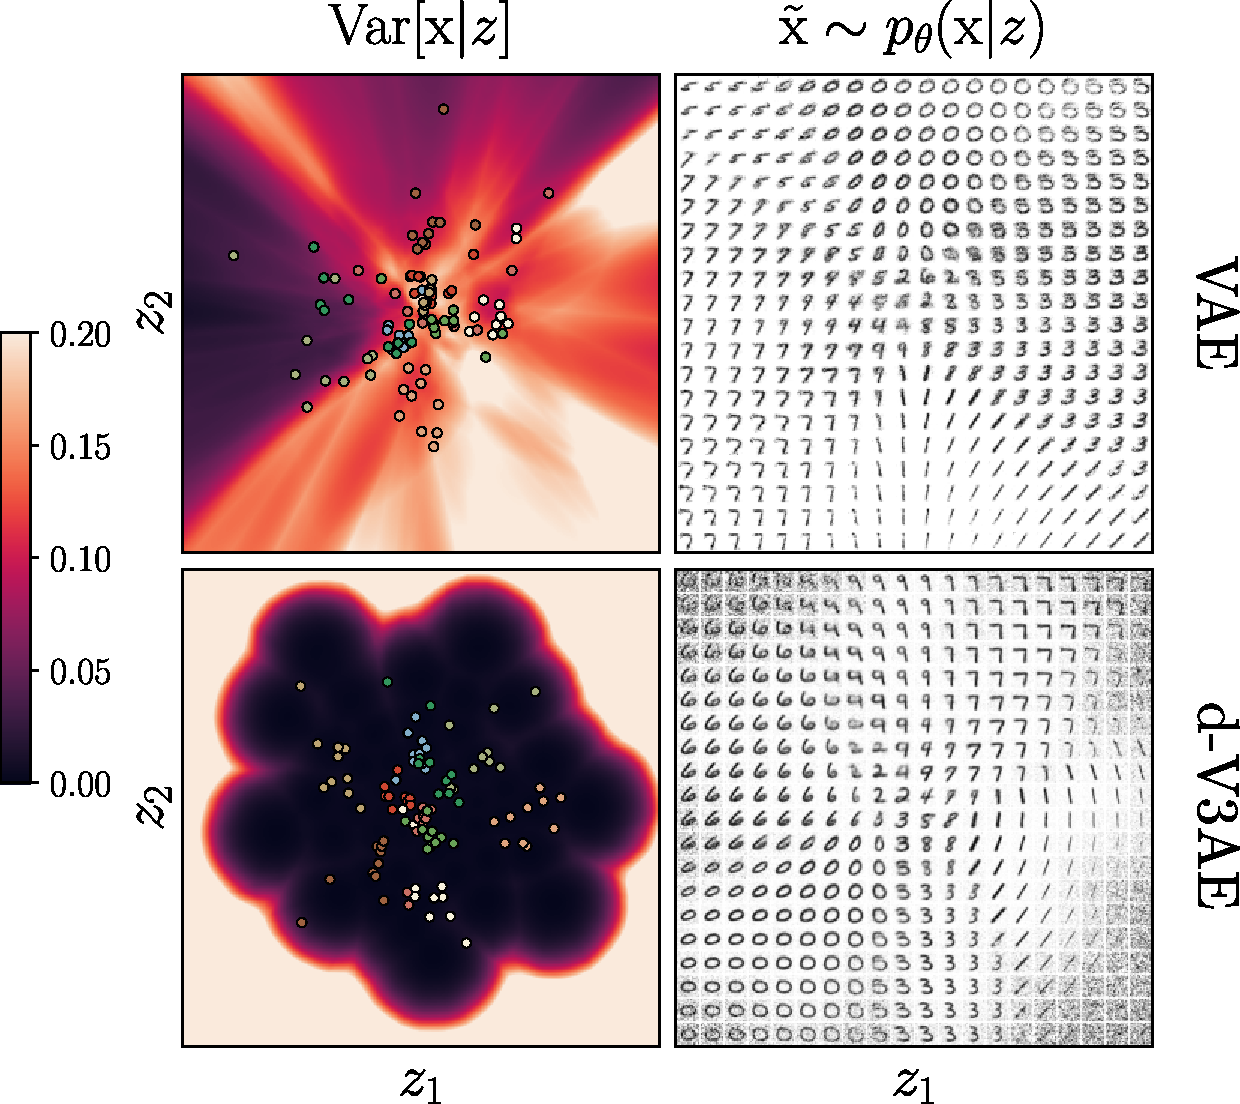
\includegraphics[height=5cm]{assets/vae_variance_plots.pdf}
        \vspace{-5.5mm}
        \captionof{figure}{Generated samples}
        \label{fig:show_vae_samples}
    \end{minipage}%
\end{figure*}